\documentclass[a4paper,12pt,oneside]{article}

% Imported packages
\usepackage[english]{babel}
\usepackage[T1]{fontenc}
\usepackage[utf8]{inputenc}
\usepackage{amssymb}
\usepackage{amsmath}
\usepackage{bm}
\usepackage{listings}
\usepackage{graphicx}
\usepackage{geometry}
\usepackage{float}
\usepackage{subfig}
\usepackage{wrapfig}
\usepackage{color}
\usepackage{comment}
\usepackage{hyperref}

% Margin dimensions settings
\geometry{a4paper,top=2cm,bottom=2cm,left=2cm,right=2cm,
	heightrounded,bindingoffset=5mm}

% Enumeration settings
\renewcommand{\thesection}{\arabic{section})}
\renewcommand{\thesubsection}{\arabic{section}\alph{subsection})}

% x bar for UTF-8 encoding
\DeclareUnicodeCharacter{304}{$ \bar{x} $}

% Code visualization settings
\lstset{basicstyle=\small\ttfamily}

% Code design settings
\lstset{language=Matlab}

% Included images path
\graphicspath{{Images/}}

% Document information
\title{Fundamentals of Vibration Analysis and Vibroacoustics \\
	Module 2 - Vibroacoustics of Musical Instruments \\
	Assignment 2 - Experimental modal analysis of a violin}
\author{Bombaci Nicola 10677942 \\
	Fantin Jacopo 10591775 \\
	Intagliata Emanuele 10544878}
\date{June 2020}


\begin{document}

\maketitle

\vspace{100pt}


\section{Matlab code for mode identification}

\subsection{Initial guess for minimization process}

Like we did for the modal parameter identification assignment, we first need an initial guess to start from.


\section{Software testing}




\section{Results}

\subsection{Comparison between reconstructed and experimental FRFs}

Our \textsc{Matlab} script identifies 7 modes. Considering one of the 125 input-output couples, we report the reconstructed Frequency Response Function compared to the corresponding experimental one. The numerical one provides a good approximation of the original one, following its amplitude envelope. We also remind that, in case the value of the modulus for one of the identified natural frequencies is not the maximum value in the considered frequency range, we considered the actual maximum value, and its corresponding frequency, for the reconstruction of that portion of FRF. This is the case for the last peak in the showed diagram, whose frequency is $ 884 \, \text{Hz} $ in place of $ 814 \, \text{Hz} $.

\begin{figure}[H]
	\hspace{-70pt}
	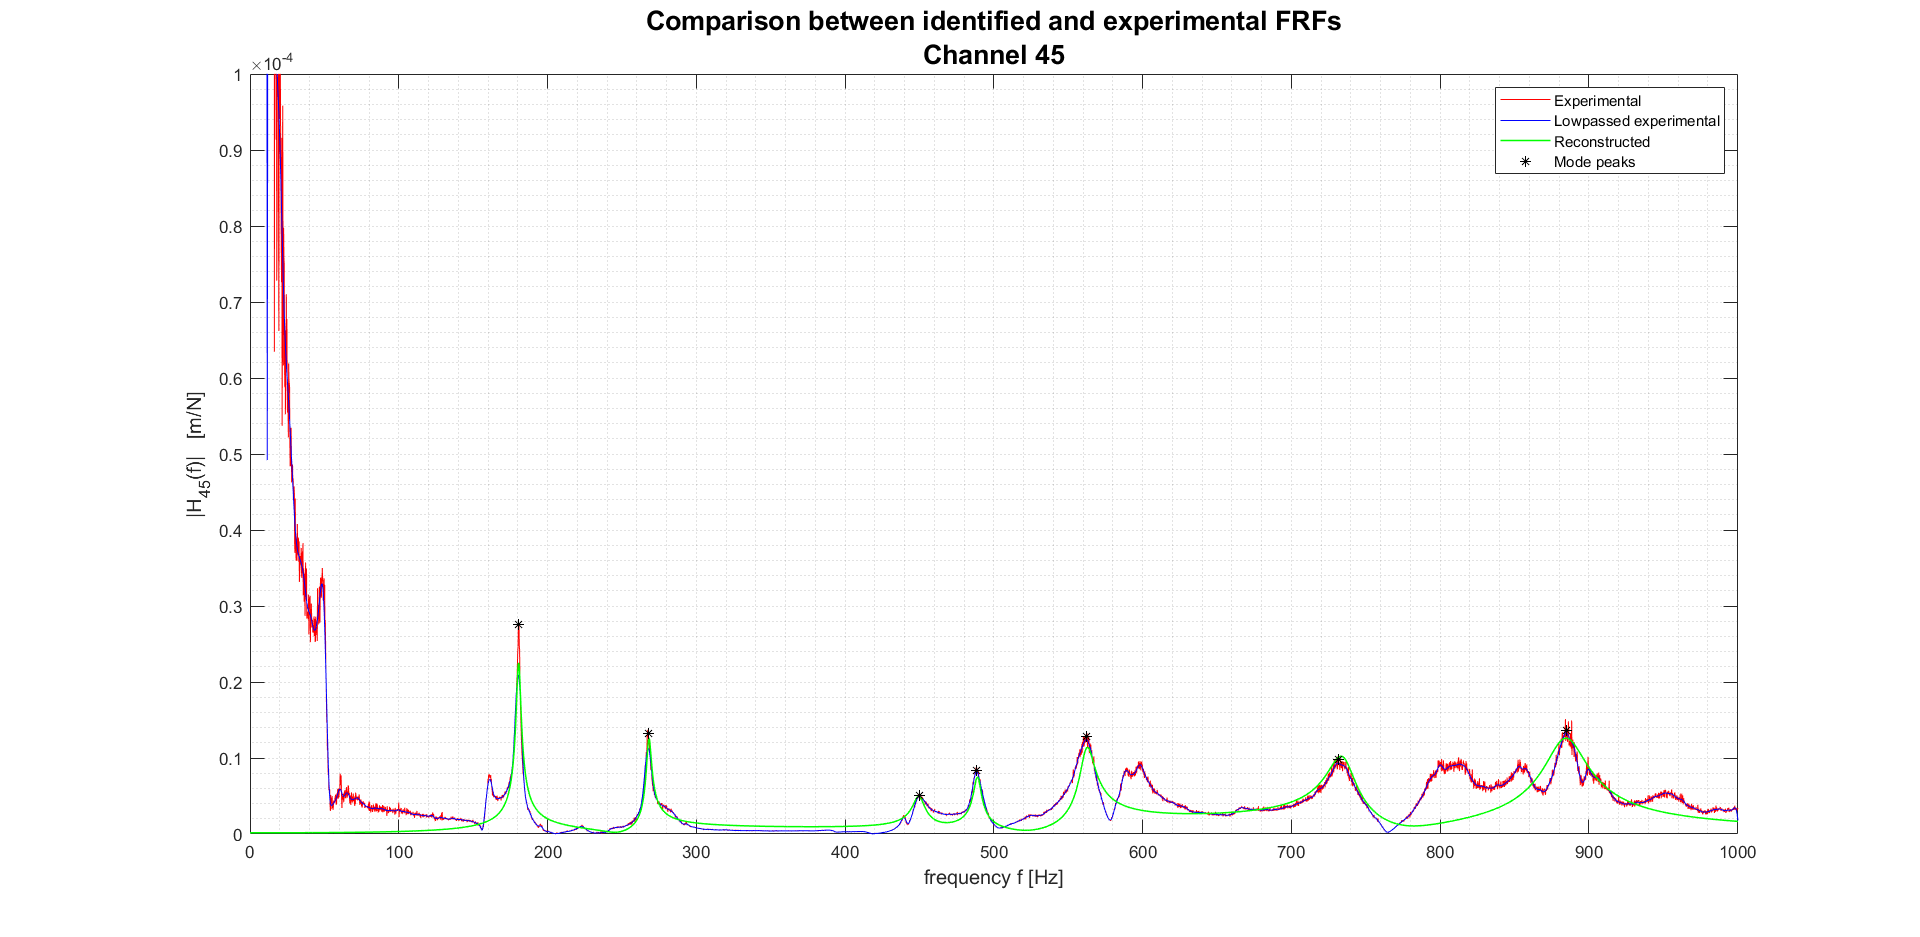
\includegraphics[scale=0.4]{frf_rec_vs_exp_ch45}
\end{figure}

Taking a closer look at each identified vibration mode, we may appreciate even more the fact a non-noisy FRF has been analitically obtained:



\subsection{Identified modes}

The following plots summarize the characteristics of the vibration modes of the violin plates: for each of them, we're displaying natural frequency, adimensional damping ratio (percentage) and a graphical representation of the mode shape, indicating the displacement of the points on the surface with respect to each other for that particular oscillation mode.

\begin{figure}[H]
	\subfloat{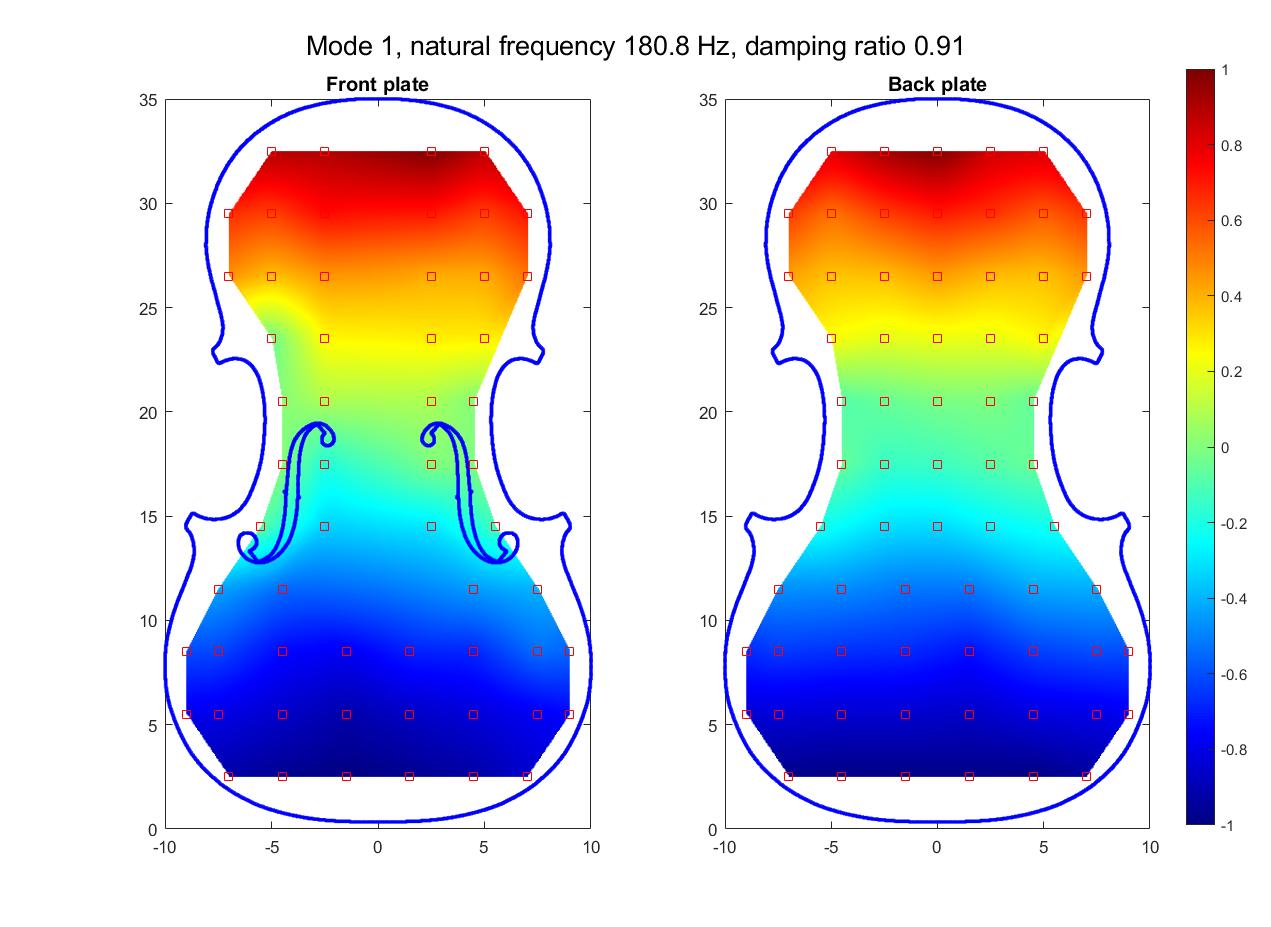
\includegraphics[scale=0.25]{mode_1}} \quad
	\subfloat{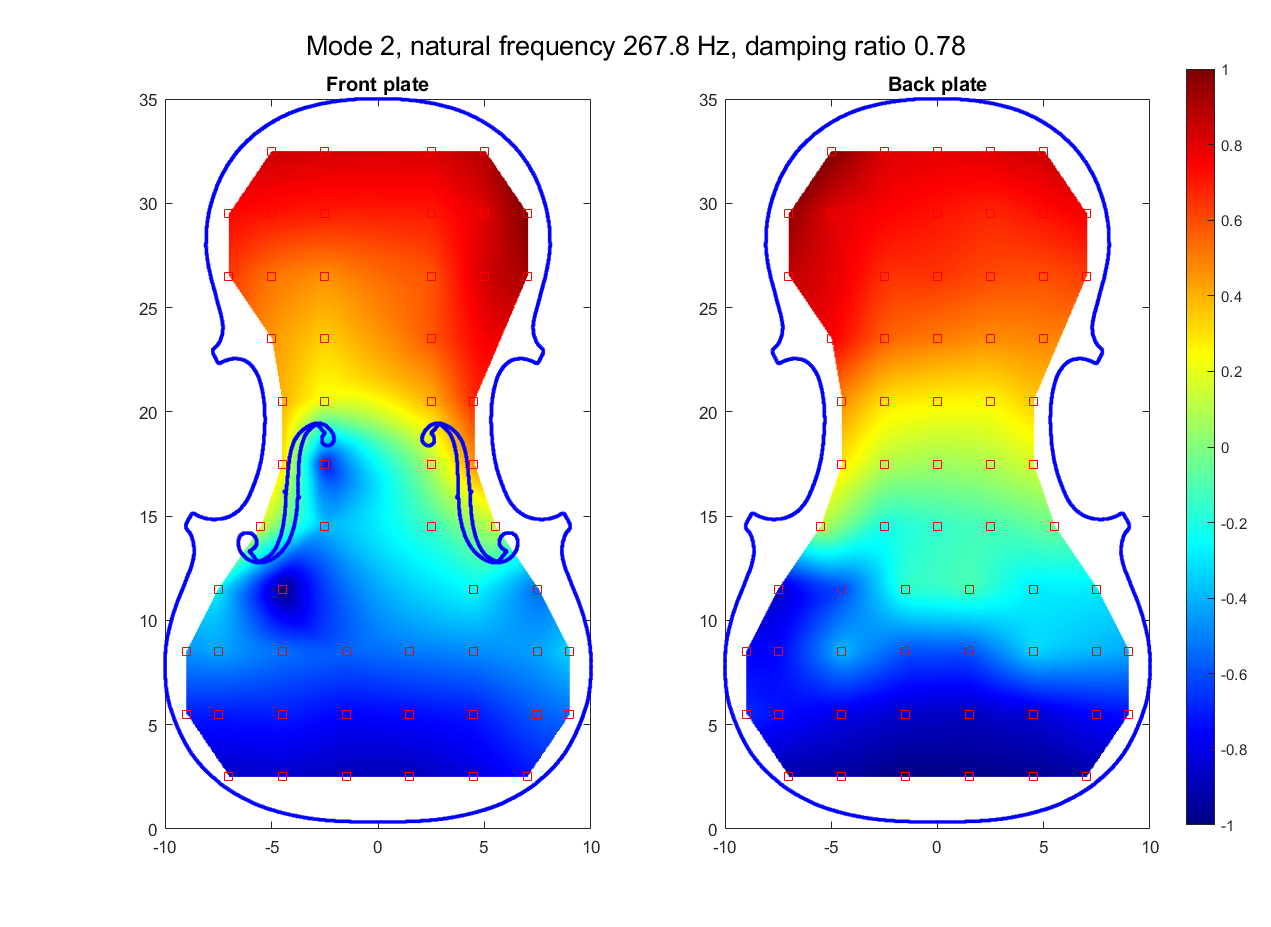
\includegraphics[scale=0.25]{mode_2}} \\
	\subfloat{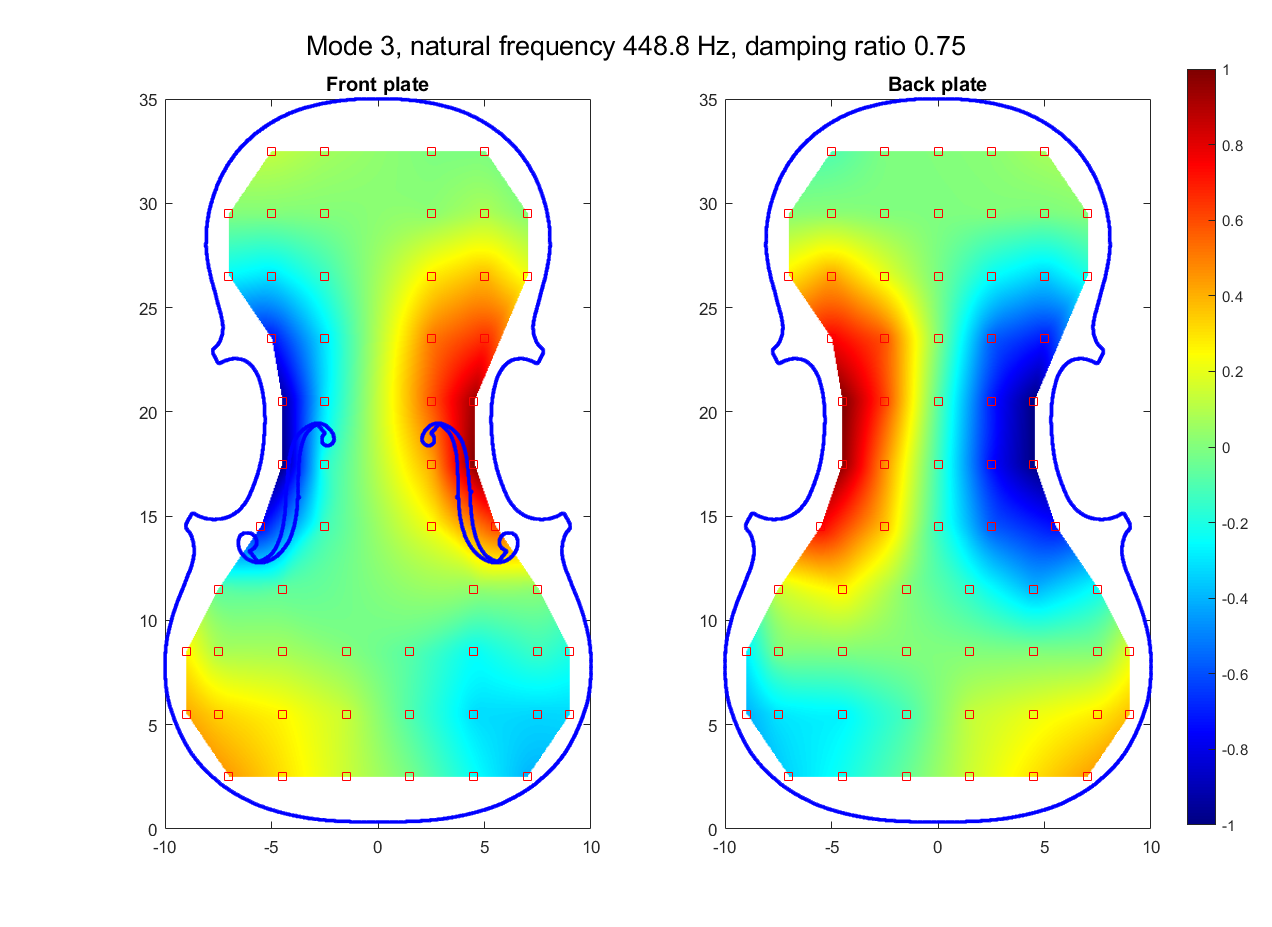
\includegraphics[scale=0.25]{mode_3}} \quad
	\subfloat{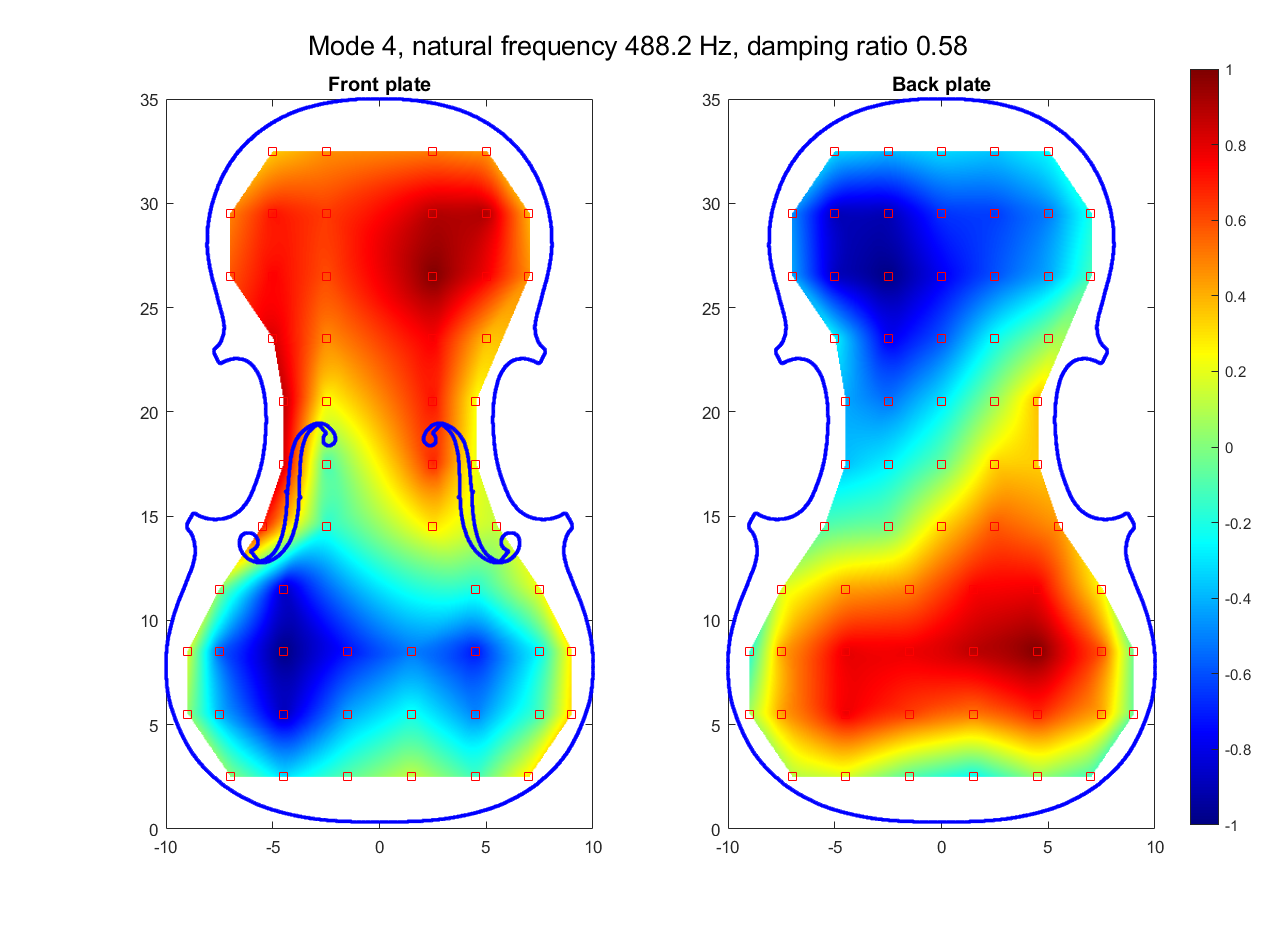
\includegraphics[scale=0.25]{mode_4}} \\
	\subfloat{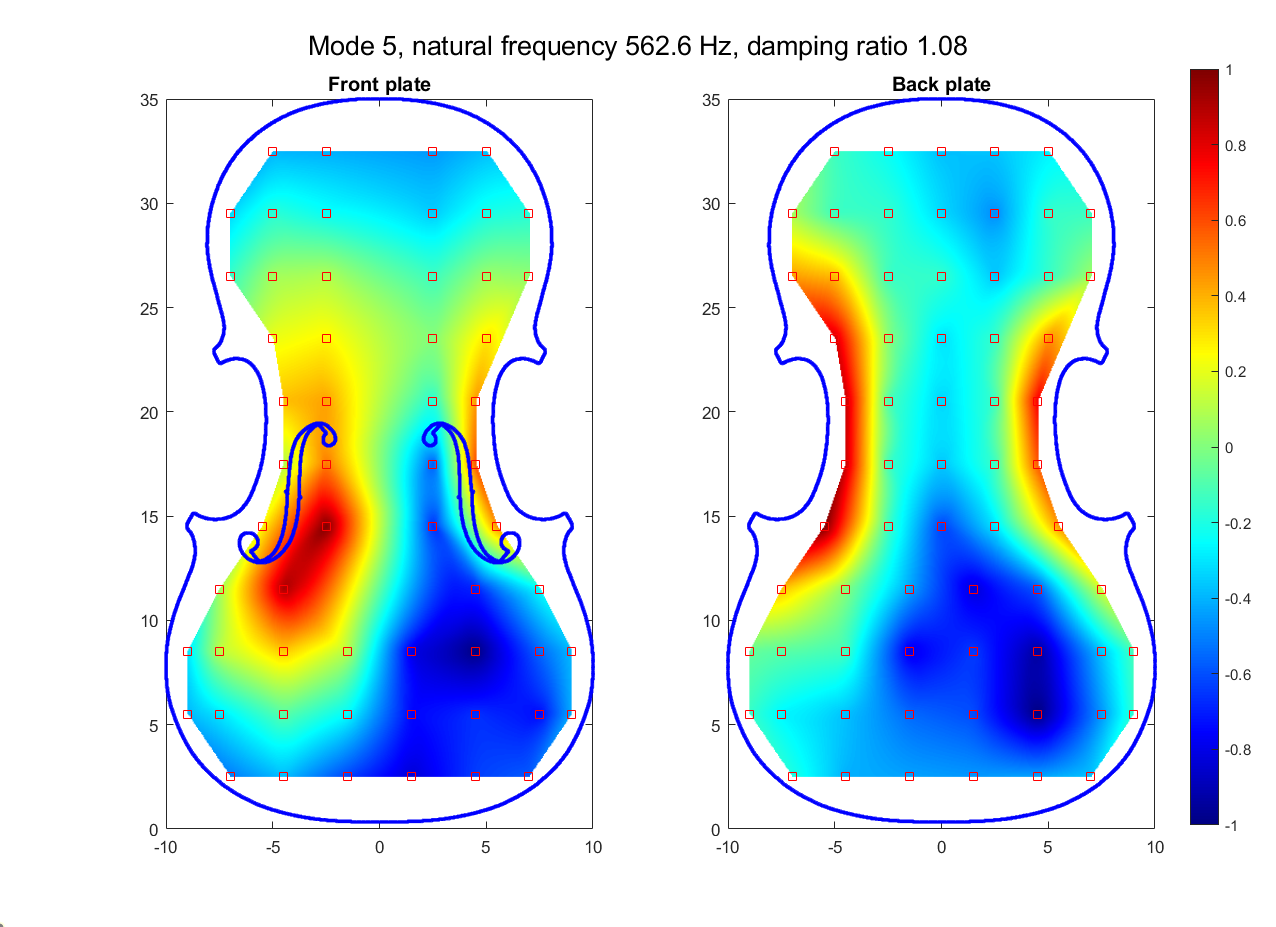
\includegraphics[scale=0.25]{mode_5}} \quad
	\subfloat{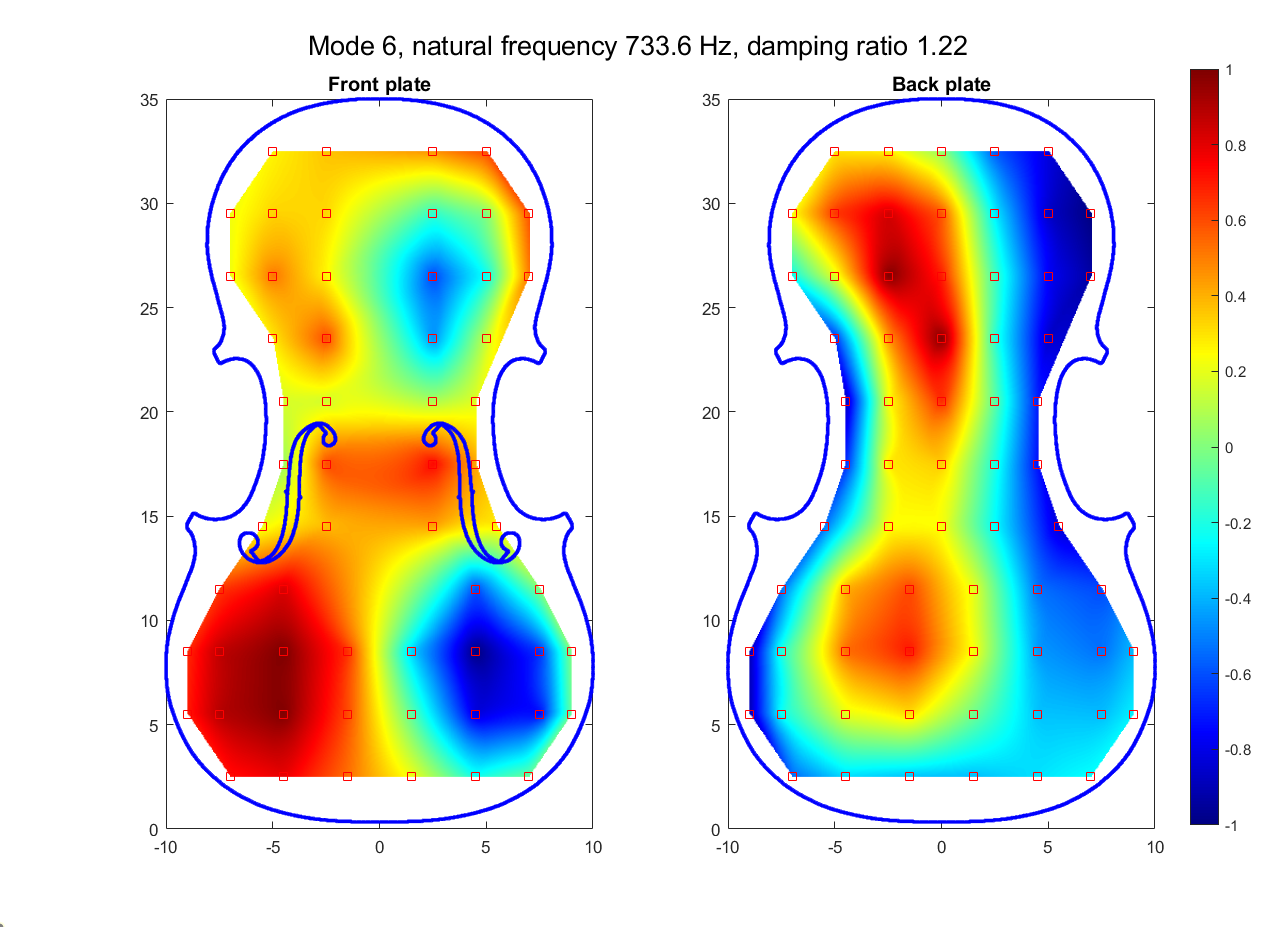
\includegraphics[scale=0.25]{mode_6}} \\
	\begin{center}
		\subfloat{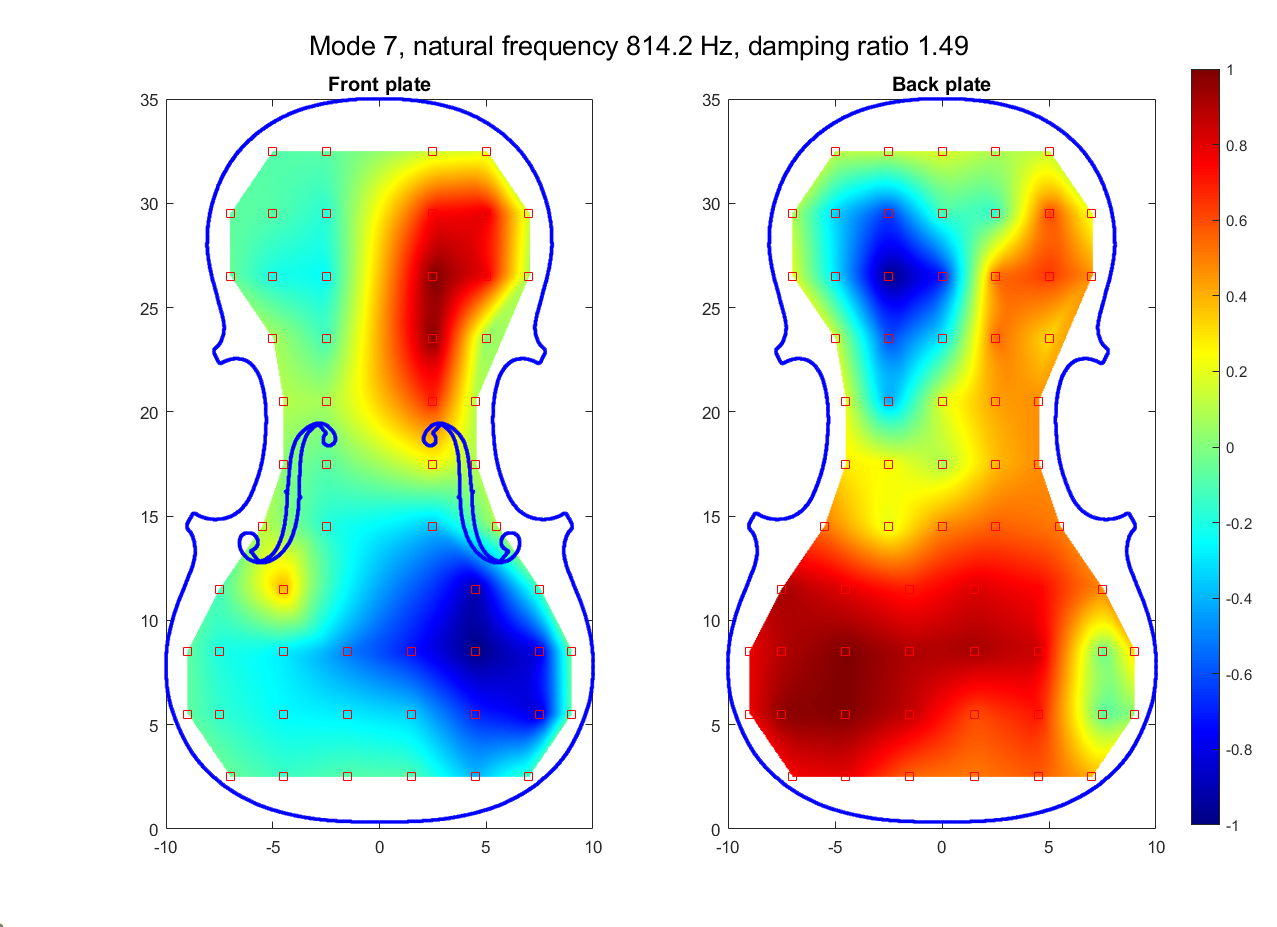
\includegraphics[scale=0.25]{mode_7}}
	\end{center}
\end{figure}

As we could infer a priori, the mode shape is more and more complex as the resonating frequency increases: in the first two modes, we can easily identify two main oscillating areas (the upper part and the lower part of the plate), in accordance between top and back plate. In the third one, there are four, with crossed polarization and accordance between top and back plate, and so on. As the mode number increases, the two plates start decouple one from the other, and the oscillation modes may not correspond anymore. This is due to the fact the higher the frequencies, the more top and back plate exhibit different modes. Talking about the damping ratio, this is on average lower at lower frequencies than at higher ones.


\end{document}